\documentclass[border=10pt]{standalone}
\usepackage[svgnames]{xcolor}
\usepackage{amsmath}
\usepackage{pgfplots}
\pgfplotsset{compat=newest}
\usepackage[sfdefault]{FiraSans}
\usepackage{FiraMono}
\renewcommand*\familydefault{\sfdefault}
\begin{document}
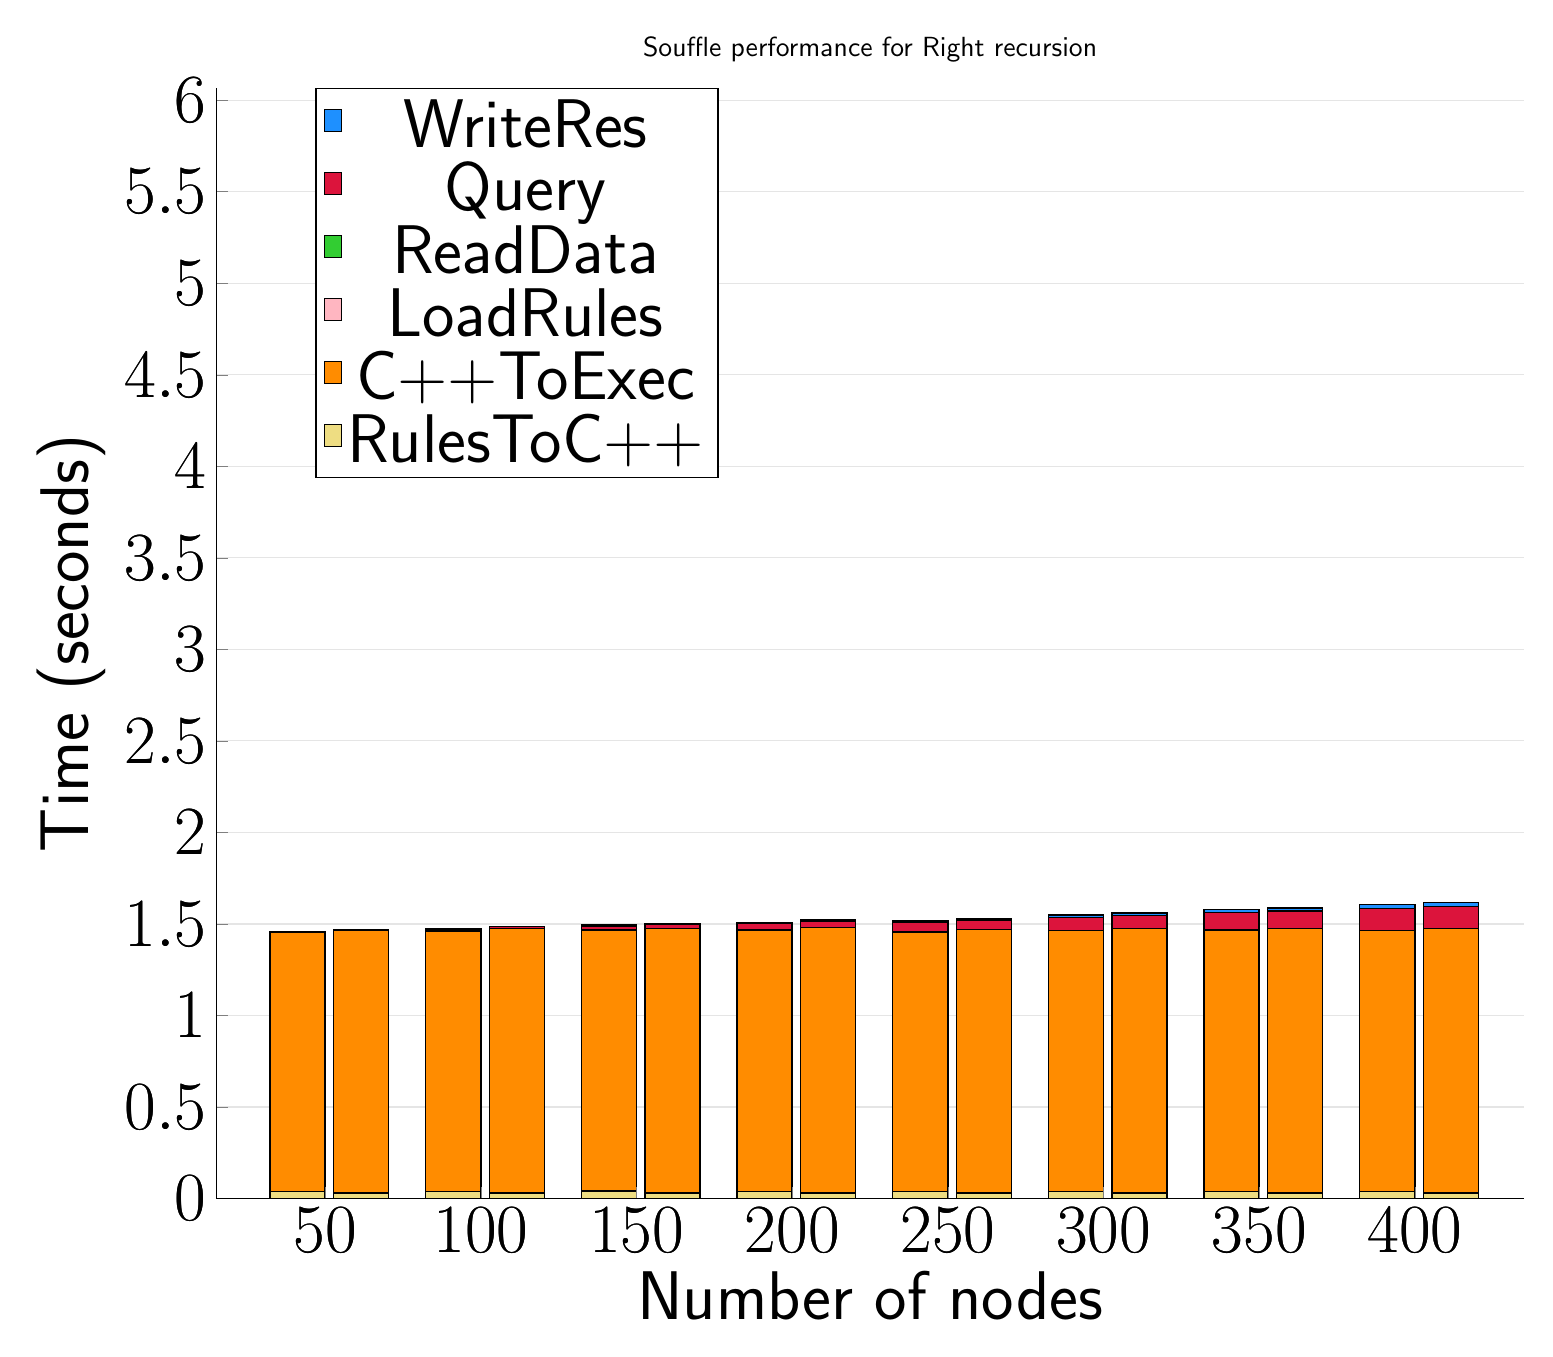
\begin{tikzpicture}
\begin{axis}[
   ybar stacked,
   title={Souffle performance for Right recursion},
   bar shift=-10pt,
   width=1.5\textwidth,
   bar width=0.7cm,
   ymajorgrids, tick align=inside,
   major grid style={draw=gray!20},
   xtick=data,
   ymin=0, ymax=6.067577,
   axis x line*=bottom,
   axis y line*=left,
   enlarge x limits=0.1,
   legend style={
       at={(0.23, 1)},
       anchor=north,
       legend columns=1,
       font=\Huge,
   },
   ylabel={Time (seconds)},
   xlabel={Number of nodes},
   label style={font=\Huge},
   tick label style={font=\Huge},
]
\addlegendimage{fill=DodgerBlue, draw=black, line width=0.2pt}
\addlegendentry{WriteRes}
\addlegendimage{fill=Crimson, draw=black, line width=0.2pt}
\addlegendentry{Query}
\addlegendimage{fill=LimeGreen, draw=black, line width=0.2pt}
\addlegendentry{ReadData}
\addlegendimage{fill=LightPink, draw=black, line width=0.2pt}
\addlegendentry{LoadRules}
\addlegendimage{fill=DarkOrange, draw=black, line width=0.2pt}
\addlegendentry{C++ToExec}
\addlegendimage{fill=LightGoldenrod, draw=black, line width=0.2pt}
\addlegendentry{RulesToC++}
\addplot +[fill=LightGoldenrod, draw=black, line width=0.5pt] coordinates {
    (50, 0.039999985694885255)
    (100, 0.04000005722045898)
    (150, 0.040999984741210936)
    (200, 0.039999985694885255)
    (250, 0.04000003337860107)
    (300, 0.04000000953674317)
    (350, 0.03899996280670166)
    (400, 0.040000104904174806)
};
\addplot +[fill=DarkOrange, draw=black, line width=0.5pt] coordinates {
    (50, 1.4120000362396241)
    (100, 1.421999955177307)
    (150, 1.4269999980926513)
    (200, 1.4259999990463257)
    (250, 1.4170000076293945)
    (300, 1.4240000009536744)
    (350, 1.428000020980835)
    (400, 1.4239999055862427)
};
\addplot +[fill=LightPink, draw=black, line width=0.5pt] coordinates {
    (50, 1.115e-05)
    (100, 1.11333e-05)
    (150, 0.0)
    (200, 1.11833e-05)
    (250, 0.0)
    (300, 2.0487499999999997e-05)
    (350, 1.11333e-05)
    (400, 2.16083e-05)
};
\addplot +[fill=LimeGreen, draw=black, line width=0.5pt] coordinates {
    (50, 0.0004251084)
    (100, 0.0005622590000000001)
    (150, 0.0006276833)
    (200, 0.0008058996000000001)
    (250, 0.0007986460000000001)
    (300, 0.0009409751000000001)
    (350, 0.0010718745)
    (400, 0.0010958991999999999)
};
\addplot +[fill=Crimson, draw=black, line width=0.5pt] coordinates {
    (50, 0.002132647)
    (100, 0.009201801)
    (150, 0.02086029)
    (200, 0.03510054)
    (250, 0.049533139999999996)
    (300, 0.07209618999999999)
    (350, 0.09525927000000001)
    (400, 0.1198262)
};
\addplot +[fill=DodgerBlue, draw=black, line width=0.5pt] coordinates {
    (50, 0.0007550832)
    (100, 0.002196508)
    (150, 0.005057795)
    (200, 0.006742058999999999)
    (250, 0.009448709)
    (300, 0.01278964)
    (350, 0.017115889999999998)
    (400, 0.02251096)
};
\end{axis}
\begin{axis}[
   ybar stacked,
   bar shift=13pt,
   width=1.5\textwidth,
   bar width=0.7cm,
   ymajorgrids, tick align=inside,
   major grid style={draw=none},
   xtick=data,
   ymin=0, ymax=6.067577,
   axis x line*=none,
   axis y line*=none,
   enlarge x limits=0.1,
   label style={font=\Huge},
   tick label style={font=\Huge},
]
\addplot +[fill=LightGoldenrod, draw=black, line width=0.5pt] coordinates {
    (50, 0.030000000000000006)
    (100, 0.031)
    (150, 0.030000000000000006)
    (200, 0.030000000000000006)
    (250, 0.030000000000000006)
    (300, 0.030000000000000006)
    (350, 0.030000000000000006)
    (400, 0.030000000000000006)
};
\addplot +[fill=DarkOrange, draw=black, line width=0.5pt] coordinates {
    (50, 1.4349999999999998)
    (100, 1.4449999999999998)
    (150, 1.4459999999999997)
    (200, 1.4499999999999997)
    (250, 1.4389999999999996)
    (300, 1.4449999999999996)
    (350, 1.4439999999999995)
    (400, 1.4449999999999996)
};
\addplot +[fill=LightPink, draw=black, line width=0.5pt] coordinates {
    (50, 1.11e-05)
    (100, 1.1e-05)
    (150, 0.0)
    (200, 1.1e-05)
    (250, 0.0)
    (300, 0.0)
    (350, 1.1e-05)
    (400, 2.14e-05)
};
\addplot +[fill=LimeGreen, draw=black, line width=0.5pt] coordinates {
    (50, 0.000411)
    (100, 0.0004953999999999999)
    (150, 0.0006119999999999999)
    (200, 0.0007427)
    (250, 0.0007319999999999999)
    (300, 0.0009214)
    (350, 0.0010491)
    (400, 0.0010789)
};
\addplot +[fill=Crimson, draw=black, line width=0.5pt] coordinates {
    (50, 0.0021315999999999996)
    (100, 0.009199599999999999)
    (150, 0.020832)
    (200, 0.03505219999999999)
    (250, 0.049353999999999995)
    (300, 0.0719398)
    (350, 0.09511539999999999)
    (400, 0.1196245)
};
\addplot +[fill=DodgerBlue, draw=black, line width=0.5pt] coordinates {
    (50, 0.0007411000000000001)
    (100, 0.0021907)
    (150, 0.0043235)
    (200, 0.006561699999999999)
    (250, 0.009152799999999999)
    (300, 0.012706899999999998)
    (350, 0.0170911)
    (400, 0.0223557)
};
\end{axis}
\end{tikzpicture}

\end{document}
